\chapter[A Parameter Space Exploration of Dust Formation]{A Parameter Space Exploration of Dust Formation within WCd Systems Using an Advected Scalar Dust Model}


\begin{abstract}
    
\end{abstract}

\section{Introduction}


Binary systems with colliding stellar winds are a fascinating phenomena capable of producing a variety of phenomena, the shock produced from these interacting systems is one of the most luminous persistent stellar-mass X-ray sources in the night sky, 
\parencite{usov_stellar_1991}, within the wind collision region the available mechanical energy rivals the radiative energy of many stars, producing shocks with temperatures exceeding $10^8$ \si{\kelvin} with densities approximately 4 orders of magnitude higher than the local medium.

Despite this, in particularly energetic Colliding Wind Binary\footnote{CWB} systems, such as those with an evolved Wolf-Rayet (in particular the WC sub-type) star as the source of the dominant wind in the system\footnote{A WR+OB binary} dust has been observed to form.
\cite{allenInfraredPhotometryNorthern1972} first attributed IR excess around WC systems to dust in the form of amorphous carbon grains; however, the high wind temperatures and extremely high luminosities around WC systems is such that dust grains would be readily destroyed through sublimation processes.
Despite this, dust has been observed to form readily in binary systems\footnote{WCd system}, even with an additional highly luminous star and a shock that would quickly destroy dust acting upon these nascent, fragile dust grains.
The exact mechanisms of dust formation as well as the evolution of dust within these systems is poorly understood, however dust formation rates can be extremely high, up to $10^{-8}$ \si{\solarmass\per\year}, or approximately $0.1\%$ of the total wind by mass.

% Persistent and episodic dust forming systems
% Discuss leading theories briefly

Dust has also been observed forming either consistently and periodically within different colliding wind binary systems.
Whilst the exact mechanism for this condition is not currently known, there is a strong correlation between periodicity and eccentricity, with more circularly orbiting systems exhibiting 
Due to this orbital dependency, it is likely that there is an optimal dust forming separation, where dust can form in large quantities. This could be due to factors such as strong post shock cooling, which is highly dependent on the wind speed and orbital separation.
Additionally, dust may be protected from the bulk of the stellar radiation due to the extremely large degree of extinction from the dense post-shock environment.

% Why is it so hard to observe these systems?

Direct observation of dust forming CWB, in particular the Wind Collision Region\footnote{WCR} is exceptionally difficult for a number of reasons:

\begin{itemize}
  \item WR+OB CWB systems are extremely rare, with $< 100$ systems having been detected within the Milky Way.
  \item Not all WC+OB systems are dust producing, limiting the sample size further.
  \item Galactic WCR systems are comparatively distant from earth, WR 104, a well-studied system, is at a distance of $\sim 2.5$ \si{\kilo\parsec}, this prevents observations of these systems at a high angular resolution.
  \item The surrounding dust cloud and high densities of the WCR introduce extreme levels of extinction, limiting visible light observations of these systems.
  \item Based on observations of CWB systems (//TODO cite this) it appears that initial grain growth is quite rapid, this means that studying the evolution of dust as it travels through the system is exceedingly difficult.
\end{itemize}

Numerical simulations, for these reasons, are ideal for modelling the growth of dust grains within this unresolved region.

% Proposal of work, what is this project covering?

In order to better understand what influences dust production in a CWB system, a parameter space exploration of the wind and orbital parameters was performed.
In particular the orbital separation, mass-loss rate and wind velocity were modified for both stars in order to influence the wind momentum ratio, $\eta$, and the cooling parameter, $\chi$.

% Discussion of parameters, eta and chi

The wind momentum ratio is a measure of the imbalance between the two winds, given as the ratio of the total wind momenta of both stars in the system:

\begin{equation}
  \eta = \frac{\dot{\text M}_\text{OB} v^\infty_\text{OB}}{\dot{\text M}_\text{WR}v^\infty_\text{WR}} ,
\end{equation}

where $\dot{\text{M}}$ is the mass loss rate of a star, while $v^\infty$ is the terminal velocity of a stars outflow.
A low value for $\eta$ indicates that the winds are extremely imbalanced, with one star dominating the wind dynamics of the system.
The wind momentum ratio can also be used to provide an approximation of the dynamics of the system, for a given orbital separation, $d_\text{sep}$ the distance from each star to the apex of the wind collision region shock can be estimated with the formulae:

\begin{subequations}
  \begin{align}
    r_\text{WR} & = \frac{1}{1+\eta^{1/2}} d_\text{sep} , \\
    r_\text{OB} & = \frac{\eta^{1/2}}{1+\eta^{1/2}} d_\text{sep} .
  \end{align}
\end{subequations}

In the case of a very small wind momentum ratio the primary stars wind completely envelopes the secondary stars forming a strong shock front; the geometry of which can be approximated in the form of a conic surface with an opening angle, $\theta$,

\begin{equation}
  \theta \simeq 2.1 \left( 1 - \frac{\eta^{2/5}}{4}\right) \eta^{-1/3} ~~~ \text{for} ~ 10^{-4} \leq \eta \leq 1 ,
\end{equation}

to a high degree of accuracy \parencite{eichler_particle_1993}.

The cooling parameter, $\chi$, compares the cooling time to the escape time from the shock region for a parcel of gas in the immediate post-shock environment. An approximation can be made using the known parameters of a system using the equation:

\begin{equation}
    \chi = \frac{t_\text{cool}}{t_\text{esc}} \approx \frac{v_8^4 d_{12}}{\dot{\text M}_{-7}} , 
\end{equation}

where $v_8$ is the wind terminal velocity in units of $10^8$ \si{cm.s^{-1}}, $d_{12}$ is the distance to the WCR apex in units of $10^{12}$ \si{cm}, and $\dot{\text M}_{-7}$ is the mass loss rate in units of $10^{-7} \si{\solarmass\per\year}$ \parencite{stevens_colliding_1992}.
Small values of $\chi$ indicate that radiative cooling dominates the dynamics of the system, while larger values indicate an adiabatic system.
Strong cooling occurs in comparatively slow, dense winds with a high metallicity, as such it can be predicted that the post-shock WR flow will rapidly cool from the immediate post-shock temperature of $10^8 \, \si{\kelvin}$ to temperatures in the dust formation range, $\lesssim 10^4 \, \si{\kelvin}$.

%//TODO Quick section on why this is important

\section{Methodology}

Numerical simulations within this paper utilise the Athena++ hydrodynamical code, a highly modular modern fluid dynamics code \parencite{stoneAthenaAdaptiveMesh2020}.
Simulations are generated in 3D and the Euler hydrodynamical equations are solved in the form:

\begin{subequations}
  \begin{align}
    \frac{\partial\rho}{\partial t}+\nabla \cdot \left(\rho \boldsymbol{u}\right) & = 0 , \\
    \frac{\partial \rho \boldsymbol{u}}{\partial t} + \nabla \cdot \left(\rho \boldsymbol{u} u + P \right) & = 0, \\
    \frac{\partial \rho \varepsilon}{\partial t} + \nabla \cdot \left[ \boldsymbol{u} \left( \rho\varepsilon + P \right) \right] & = \dot E_{cool} , 
  \end{align}
\end{subequations}

where $\varepsilon$ is the total specific energy, $\varepsilon = \boldsymbol{u}^2/2 + e/\rho $, $\rho$ is the mass density, $e$ is the internal energy density, $P$ is the gas pressure and $u$ is the gas velocity.
In order to simulate radiative losses, the parameter $\dot E_{cool}$ is included, which is the energy loss rate from the fluid due to gas and dust cooling, which is elaborated on in section \ref{sec:gas-dust-cooling}.

% Technical details

Athena++ has been configured to run using a piecewise linear reconstruction method with a 4\ts{th} order Strong Stability Preserving Runge-Kutta time-integration method \parencite{spiteriNewClassOptimal2002}.
Athena++ was forked from the original repository and additional routines were written for a Colliding Wind Binary case.
To simulate the dynamics of the simulation functions were created to produce a steady outflow from a small spherical region around a set of cartesian co-ordinates as well as a function to move these co-ordinates with each time-step; these were used to simulate stellar wind outflow orbital motion respectively.
Additionally, Athena++ was further modified to include an advected scalar dust model for simulating dust growth and destruction as well as a photon emission cooling model to approximate cooling for gas and dust particles within the fluid.
Athena++ utilises OpenMPI for parallelism, breaking the simulation into blocks, which are distributed between processors, the block size is variable, but for these simulations a block size of $32\times 32 \times 8$ was found to be optimal.
This meshblock system is also utilised in mesh refinement for increasing effective resolution.
As the CWB systems are being simulated in their entirety, a very large area needs to be simulated, while at the same time the region between the stars must be resolved with a resolution of at least 100 cells in order to adequately resolve the WCR.
This difference in length scales necessitates the use of static mesh refinement to improve the effective resolution of the simulation.
A base coarse resolution of $320 \times 320 \times 40$ cells is defined for the simulations, while a region close to the binary pair operates at a higher refinement level, resulting in a resolution increase with a factor of $2^{n-1}$ greater than the coarse resolution, where $n$ is the refinement level; this can be seen in figure \ref{fig:smr-grid} where .
this results in an effective resolution $20480 \times 20480 \times 2560$ cells.
SMR is utilised instead of Adaptive Mesh Refinement, a more flexible conditional method as it has proven to be more reliable within Athena++, as it mitigates unintentional over-refinement.
As much of the grain evolution occurs a small distance from the WCR stagnation point, much of the simulation can be run at a lower resolution without affecting the simulation outcome.

\begin{figure}
  \centering
  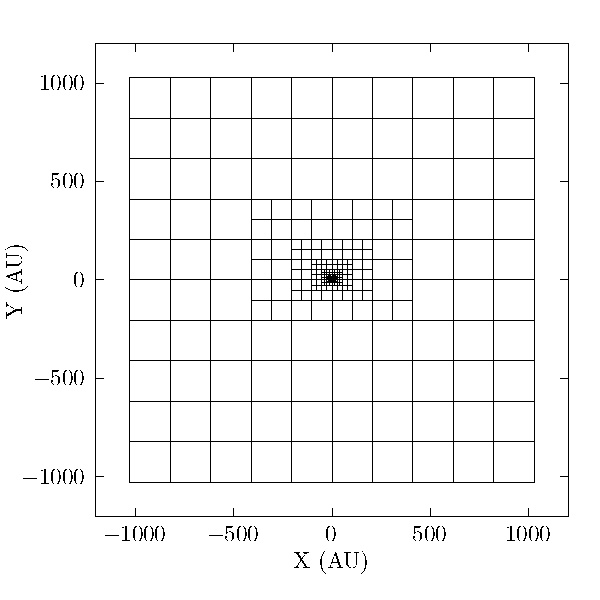
\includegraphics{assets/mesh/gridxy.pdf}
  \caption[Static mesh refinement example]{Plot of blocks used in a 7 level simulation with a block size of $32\times 32 \times 8$ cells, block density increases dramatically closer to the barycentre.}
  \label{fig:smr-grid}
\end{figure}

Wind outflow from stars is simulated by replacing the conserved values for density, momentum and energy within a small region around the expected position of the stars; this region is typically on the order of 6 maximally refined cells in radius.
This rewrite corresponds to a change in mass and mechanical energy imparted by an outflowing wind, such that:

\begin{subequations}
  \begin{align}
    \rho_R & = \frac{\dot M}{(4 \pi r^2 v_\infty)} , \\
    P_R & = \frac{\rho_R}{\mu m_H} k_B T_w , \\
    p_{R} & = \rho_R v_{R} , \\
    E_R & = \frac{P_R}{\gamma - 1} + \frac{1}{2} \rho_{R} v_{r}^2 ,
  \end{align}
\end{subequations}

% This may need more explanation, depending on previous equations

where $v_r$ is the wind velocity as it flows radially from the center of the ``remap zone'' and $r$ is the distance from the current cell to the centre of the remap zone.
Orbits are calculated by moving the remap zones in a manner consistent with Keplerian dynamics, which are updated at every timestep.

% Plasma and dust cooling

\subsection{Gas and dust cooling} \label{sec:gas-dust-cooling}

Cooling due to photon emission from gas molecules and dust particles is simulated by removing energy from a cell at each timestep.
The total energy loss is calculated by integrating the energy loss rates due to plasma and dust cooling using the Euler method; in regions with very rapid cooling sub-stepping is used to improve accuracy, with the number of sub-steps being determined by comparing the substep time to the cooling timescale of the cell.
Gas cooling is simulated using a lookup table method, a data file containing the gas temperature and associated emissivity, $\Lambda(T)$ of the wind at that temperature is read into the simulation.
In a typical cooling step, the temperature is calculated and a binary search is performed to find the nearest temperature in the lookup table, a linear interpolation step is then performed to find an appropriate value for $\Lambda$.
The emissivity is normalised for a $1 \si{cm^{-3}}$ volume with a density of $1 \si{g.cm^{-3}}$, as such, the energy loss can be calculated with the formulae:

\begin{equation}
  \frac{dE}{dt} = \left(\frac{\rho}{m_H}\right)^2 \Lambda_w(T),
\end{equation}

where $\rho$ is the gas density and $m_H$ is the mass of a hydrogen atom.
The lookup table was generated by mixing a series of cooling curves generated by MEKAL simulations of elemental gasses, these are combined based on the elemental abundances of each wind such that:

\begin{equation}
  \Lambda(T) = n_e n_i \sum{X_E \Lambda_{E}(T)},
\end{equation}

where $n_e$ and $n_i$ are the electron and ion number density of an element, $X_E$ is the abundance of an element, while $\Lambda_E(T)$ is the cooling parameter of an element.
Figure \ref{fig:cooling-curve} shows the cooling curves used for each star, as well as non-normalised emissivities for each element.
Two lookup tables are used in the simulations, based on the elemental abundances of each star. the Wolf-Rayet star uses a curve with abundances typical of a WC9 star with total hydrogen depletion and a high carbon mass fraction, while the OB star is assumed to have solar abundances.
The most significant abundances used in this projects simulations are presented in table \ref{tab:abundances}.
The cooling regime of this code ranges from $10^4$ to $10^9 \si{\kelvin}$, cooling or heating above or below these temperatures are automatically restricted.

\begin{table}
  \centering
  \begin{tabular}{@{}ccc@{}}
  \toprule
  \multicolumn{1}{l}{} & \multicolumn{2}{c}{X(E)} \\ \cmidrule(l){2-3} 
   & Solar & WC9 \\ \midrule
  H & $0.705$ & $0.0$ \\
  He & $0.275$ & $0.546$ \\
  C & $3.07 \times 10^{-3}$ & $0.4$ \\
  N & $1.11 \times 10^{-3}$ & $0.0$ \\
  O & $9.60 \times 10^{-3}$ & $0.05$ \\
  % Ne & $1.75 \times 10^{-3}$ & $0.0$ \\
  % Na & $3.47 \times 10^{-5}$ & $3.47 \times 10^{-5}$ \\
  % Mg & $7.10 \times 10^{-4}$ & $7.10 \times 10^{-4}$ \\
  % Al & $6.13 \times 10^{-5}$ & $6.13 \times 10^{-5}$ \\
  % Si & $8.60 \times 10^{-4}$ & $8.60 \times 10^{-4}$ \\
  % S & $3.82 \times 10^{-4}$ & $3.82 \times 10^{-4}$ \\
  % Ar & $1.01 \times 10^{-4}$ & $1.01 \times 10^{-4}$ \\
  % Ca & $6.15 \times 10^{-5}$ & $6.15 \times 10^{-5}$ \\
  % Fe & $1.52 \times 10^{-3}$ & $1.52 \times 10^{-3}$ \\
  % Ni & $7.65 \times 10^{-5}$ & $7.65 \times 10^{-5}$ \\ \bottomrule
  \end{tabular}
  \caption[Abundances used for OB and WR stars]{Abundances used for OB and WR stars, other elements are effectively trace.}
  \label{tab:abundances}
\end{table}


\begin{figure}[ht]
  \centering
  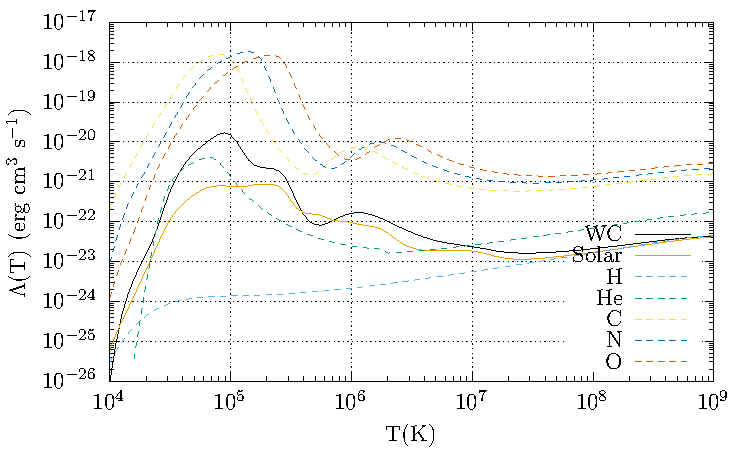
\includegraphics{assets/cooling-curve/cooling-curve.pdf}
  \caption[WR and OB $\Lambda(T)$ cooling curves]{Comparison of lookup tables for calculating energy loss due to gas cooling, pure elemental cooling curves from MEKAL have been provided for the more abundant elements.}
  \label{fig:cooling-curve}
\end{figure}

A model for cooling due to emission from dust grains is also included as dust cooling was expected to play a significant role in the evolution of each system.
The rate of cooling is calculated using the uncharged particle case of the Dwek \& Werner prescription \parencite{dwek_infrared_1981}.
Grains are heated due to collisions with ions and electrons, causing them to radiate, with energy being removed from the simulation.
This assumes that infrared emission due to collisional heating is shorter than the cooling timestep, and the region being simulated is optically thin to far infrared photons.
Ions are calculated by element by estimating their number density, with the energy loss rate calculated with the following formulae:

\begin{subequations}
  \begin{align}
    H_\text{coll} & = 1.26 \times 10^{-19} \frac{n}{A^{1/2}} a^2(\mu \text m) T^{3/2} h(a,T) , \\
        \Lambda_d & = \frac{H_\text{coll} + H_\text{el}}{n_H} , \\
    \frac{dE}{dt} & = n_T n_d \Lambda_d ,
  \end{align}
\end{subequations}

where $H_\text{coll}$ is the heating rate due to atom and ion collisions, $H_\text{el}$ is the heating rate due to electron collisions, $h(a,T)$ is the grain-ion transparency and $n_T$ is the total number density.
$H_\text{coll}$ is summated for Hydrogen, Helium, Carbon, Nitrogen and Oxygen atom collisions, other elements are not considered as they are present in trivial proportions in both winds.

Electron-grain collisions are modelled similarly to ions, albeit with some differences.
One major factor for calculating accurate energy loss due to electron collisions is that the electron number density needs to be accurately calculated; this is performed with a second series of lookup tables that contain the electron-to-ion ratio of each wind across a temperature range of $10^4$ to $10^9\si{\kelvin}$ (figure \ref{fig:electron-curve}).
The electron number density is found to be $n_e = n_e/n_i n_i$ where $n_e/n_i$ is the electron-to-ion ratio and $n_i$ is the ion number density.

\begin{figure}[h]
  \centering
  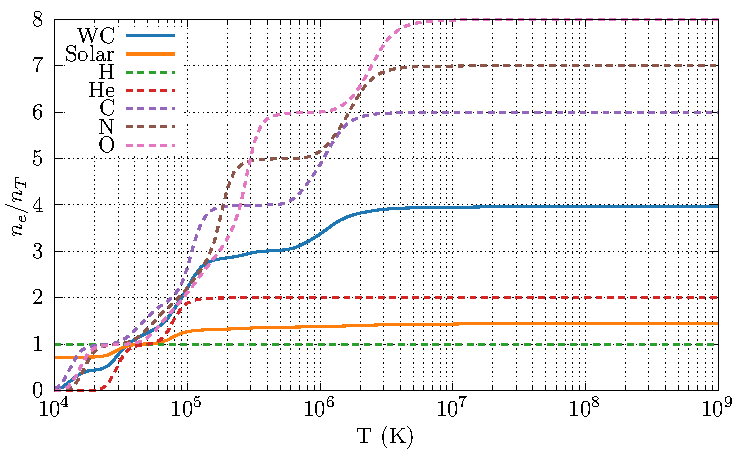
\includegraphics{assets/ionisation-fraction/ionisation-fraction.pdf}
  \caption[OB and WR electron-ion ratios]{A comparison of the electron-ion ratio of both winds as temperature changes, included are the pure wind flows that the lookup tables are built from.}
  \label{fig:electron-curve}
\end{figure}

Additionally, calculating electron-grain transparency is a significantly more complex problem than calculating ion-grain transparency.
Electron-grain transparency is calculated via an approximation described in Dwek \& Werner:

\begin{equation}
  \begin{alignedat}{3}
    h(x^*) & = 1 ,                && ~~ x^* > 4.5, \\
           & = 0.37{x^*}^{0.62} , && ~~ x^* > 1.5 , \\
           & = 0.27{x^*}^{1.50} , && ~~ \text{otherwise,}
  \end{alignedat}
\end{equation}

where $x^* = 2.71\times 10^8 a^{2/3} (\si{\micro\metre})/T$.
This approximation is approximately 4 orders of magnitude faster than using an integration method, while only being out by $\sim 8\%$ in the worst case scenario (figure \ref{fig:lambdacomparison}).

\begin{figure}
  \centering
  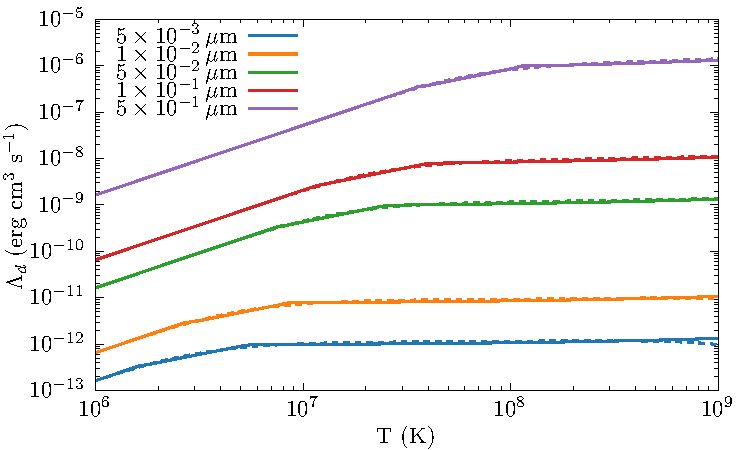
\includegraphics{assets/grain-transparency/lambda-comp.pdf}
  \caption[Comparison of electron transparency methods.]{$\Lambda_d$ as a function of temperature for various grain sizes, the estimate method is extremely close to the integral value aside from at the highest temperatures.}
  \label{fig:lambdacomparison}
\end{figure}

%//TODO this caption is the same as another one, need to come up with a new one!

Grain-grain collision is not modelled, as this would be difficult to calculate due to the single-fluid model in use, further simulations utilising a multi-fluid model could allow for this to be simulated.

% Advected scalar modification

\subsection{Numerical modelling of dust through advected scalars}

The most important modification for Athena++ was the addition of a dust growth and destruction model to simulate the production of dust within the WCR.
A passive scalar model was used where which dust can evolve and advect through the simulation, analogous to a co-moving fluid, which previous papers have noted is an accurate dynamical model for dust within the WCR \parencite{hendrix_pinwheels_2016}.
In these simulations, dust is stored in the form of two variables, the average grain radius, $a$, and the dust-to-gas mass ratio, $z$.
From these constants the dust production rate, number density, and total dust mass can be derived.
A co-moving model allows for a simplified model of dust formation. In such a model, the mean particle velocity between two particles of different size can be given as:

\begin{equation}
  \langle u \rangle = \left[ \frac{8kT}{\pi m_r} \right] ^{1/2} ,
\end{equation}

where $m_r$ is the familiar reduced mass between a test particle of mass $m_t$ and a field particle of mass $m_f$

\begin{equation}
  m_r = \frac{m_f m_t}{m_f + m_t} .
\end{equation}

As the dust grain is significantly more massive, the reduced mass is approximately equal to the grain mass, simplifying the dynamics of the simulation in a co-moving case \parencite{spitzer_jr._physical_2008}.
Dust growth is modelled through approximating growth due to grain-gas accretion, grains co-moving with a gas perform low-velocity\footnote{Relative to the overall wind velocity} collisions with the surrounding gas, accreting this gas onto the surface of the dust grain \parencite{spitzer_jr._physical_2008}.
Assuming a single average grain size and a relatively consistent grain number density the change in average grain radius and total dust mass density can be described in the form:

\begin{subequations}
  \begin{align}
        \frac{da}{dt} & = \frac{\xi_a \rho_{Gr} w_a}{4 \rho} , \\
    \frac{\rho_D}{dt} & = 4 \pi a^2 \rho n_D \frac{da}{dt}   , 
  \end{align}
\end{subequations}

where $w_a$ is the Maxwell-Boltzmann distribution RMS velocity, $\xi_a$ is the grain sticking efficiency, $\rho_{Gr}$ is the grain bulk density, $\rho$ is the gas density, $a$ is the dust grain radius, and $n_D$ is the grain number density.
In this paper $\xi_a$ is assumed to be $10\%$, while a bulk density analogous to amorphous carbon grains of $3.0 \, \si{g.cm^{-3}}$ is utilised.
Additionally, dust destruction is calculated via gas-grain sputtering using the Draine \& Salpeter prescription - a dust grain has a lifespan, $\tau$, which is dependent on the grain radius, as the grain loses radius proportional to its loss in mass; assuming a spherical grain, the rate of change in mass and radius can be calculated such that:

\begin{subequations}
  \begin{align}
           \tau_D & = 1 \, \text{Myr} \times \frac{a}{n_g} , \\
    \frac{da}{dt} & = - \frac{a}{\tau_D} , \\
    \frac{dm}{dt} & = -1.33 \times 10^{-13} a^2 n_g n_d \rho_{Gr} ,
  \end{align}
\end{subequations}

where $n_g$ is the gas number density \parencite{draine_destruction_1979}.

% //TODO cleanup sentence structures

In order to propagate dust through each simulation, a small initial value for the advected scalars is set in each cell in the remap zones, a minimum grain radius of $50 \, \text{\AA}$ and minimum dust-to-gas mass ratio of $10^{-8}$ is proposed.
Changing $z_{min}$ does not significantly impact the average final dust-to-gas mass ratio of the system as $z$ rapidly increases within the WCR, and only impacts the amount of dust formed outside of the WCR.

\section{Model Parameters}

For this paper, a series of simulations were run in order to determine how dust formation varies due changes in orbital separation and wind momentum ratio.
A baseline simulation with properties similar to WR98a but with simplified orbits was created, which was then modified to influence the orbital separation and wind momentum ratio.
Another set of simulations were run where the cooling mechanisms were selectively disabled, in order to understand how 
Table \ref{tab:baseline-windproperties} and \ref{tab:baseline-orbits} detail the wind and orbital parameters of the baseline simulation.
Orbital separation is modified by changing the orbital period of the simulation, while wind momentum ratio is modified by adjusting the mass loss ratio and wind terminal velocity for each star.

\begin{table}[h]
  \centering
  \begin{tabular}{cccc}
  \hline
  Parameter & WR & OB & Unit \\ \hline
  $\dot M$ & \num{5.0e-6} & \num{5.0e-8} & \si{\solarmass\per\year} \\
  $v_\infty$ & \num{1e8} & \num{2e8} & \si{cm.s^{-1}} \\
  $T_w$ & \num{1e4} & \num{1e4} & K \\
  \hline
  \end{tabular}
  \caption{Wind properties of the baseline system}
  \label{tab:baseline-windproperties}
\end{table}

\begin{table}[h]
  \centering
  \begin{tabular}{ccc}
  \hline
  Parameter & Value & Unit \\ \hline
  $M$ & 10.0 & \si{\solarmass} \\
  $d_{sep}$ & \num{5.984e13} & cm \\
  $P$ & \num{5.64e7} & s \\
  \hline
  \end{tabular}
  \caption{Baseline system orbital properties}
  \label{tab:baseline-orbits}
\end{table}

\subsection{Cooling mechanisms}

For this set of simulations, the influence of cooling was changed by varying how cooling works within the simulations.
All simulations in this set do not vary their orbital or wind parameters, which are that of the baseline system described in tables \ref{tab:baseline-windproperties} \& \ref{tab:baseline-orbits}, the main differing factor between simulations is the avenues available for cooling, the main simulation has both plasma and dust cooling in operation, while the other two simulations have plasma cooling only and no cooling respectively (table \ref{tab:cooling-param}).
The final, no radiative cooling simulation instead relies on adiabatic expansion for temperature change; as such, this simulation behaves as if it has a $\chi$ value for both winds that is arbitrarily high.
These simulations were performed in order to test the temperature response of the dust model, to ensure the stability of the cooling models, and to determine the role of cooling itself in the formation of dust.

% Discuss why this is important, mention overdensity due to radiative cooling

\begin{table}[h]
  \centering
  \begin{tabular}{ccc}
    \hline
    Name & Plasma cooling & Dust cooling \\
    \hline
    \texttt{fullcool} & Yes & Yes \\ 
    \texttt{plasmacool} & Yes & No \\
    \texttt{nocool} & No & No \\
    \hline
  \end{tabular}
  \caption{Cooling series simulation parameters}
  \label{tab:cooling-param}
\end{table}

\subsection{Wind momentum ratio}

A second set of simulations were devised in order to determine the role $\eta$ has on the formation of dust.
These simulations have similar orbital properties to the baseline simulation, but with varying wind properties.
$\eta$ is varied from 0.01 to 0.04 by adjusting the wind parameters for each star, this experiment is further subdivided by which property is modified, either the mass loss rate or wind terminal velocity.
Multiple simulations have similar momentum ratios and cooling parameters, but accomplished via different means, such as changing the secondary star wind rather than the primary. This is done in order to determine whether dust production changes are due to these two parameters or to the momentum ratio itself.
These simulations are also compared to the baseline simulation, which has a momentum ratio of 0.02.
These simulations were run out to a minimum of 1 orbit, with some simulations run out further to rule out the role of orbital position and simulation advection, as the results should be consistent across multiple orbits. 

\begin{table}[h]
  \centering
  \begin{tabular}{ccccccc}
  \hline
  Name & $\dot M_{WR}$ & $\dot M_{OB}$ & $v^\infty_{WR}$ & $v^\infty_{OB}$ & $\eta$ & $\chi_{WR}$ \\ 
  & \si{\solarmass\per\year} & \si{\solarmass\per\year} & \si{\centi\metre\per\second} & \si{\centi\metre\per\second} & & \\ \hline
  \texttt{baseline}& \num{5.0e-6} & \num{5.0e-8} & \num{1e8} & \num{2e8} & 0.02 & 1.049 \\
  \texttt{mdot-1}& \num{1.0e-5} & \num{5.0e-8} & \num{1e8} & \num{2e8} & 0.01 & 0.544 \\
  \texttt{mdot-2}& \num{2.5e-6} & \num{5.0e-8} & \num{1e8} & \num{2e8} & 0.04 & 1.995 \\
  \texttt{mdot-3}& \num{5.0e-6} & \num{1.0e-7} & \num{1e8} & \num{2e8} & 0.04 & 0.997 \\
  \texttt{mdot-4}& \num{5.0e-6} & \num{2.5e-8} & \num{1e8} & \num{2e8} & 0.01 & 1.088 \\
  \hline
  \end{tabular}
  \caption[Mass loss rate series wind parameters]{Wind parameters for simulations varying the mass loss rate, $\dot M$.}
  \label{tab:mdot-param}
\end{table}

\begin{table}[h]
  \centering
  \begin{tabular}{ccccccc}
  \hline
  Name & $\dot M_{WR}$ & $\dot M_{OB}$ & $v^\infty_{WR}$ & $v^\infty_{OB}$ & $\eta$ & $\chi_{WR}$ \\ 
  & \si{\solarmass\per\year} & \si{\solarmass\per\year} & \si{\centi\metre\per\second} & \si{\centi\metre\per\second} & & \\ \hline
  \texttt{baseline} & \num{5e-6} & \num{5e-8} & \num{1e8} & \num{2e8} & 0.02 & 1.049 \\
  \texttt{vinf-1} & \num{5e-6} & \num{5e-8} & \num{2e8} & \num{2e8} & 0.01 & 17.41 \\
  \texttt{vinf-2} & \num{5e-6} & \num{5e-8} & \num{5e7} & \num{2e8} & 0.04 & 0.062 \\
  \texttt{vinf-3} & \num{5e-6} & \num{5e-8} & \num{1e8} & \num{4e8} & 0.04 & 0.997 \\
  \texttt{vinf-4} & \num{5e-6} & \num{5e-8} & \num{1e8} & \num{1e8} & 0.01 & 1.088 \\
  \hline
  \end{tabular}
  \caption[Terminal velocity series wind parameters]{Wind parameters for simulations varying the wind terminal velocity, $v^\infty$.}
  \label{tab:vinf-param}
\end{table}

\subsection{Separation distance}

A final series of simulations was performed with a binary pair utilising wind parameters described in table \ref{tab:baseline-windproperties} with a differing orbital separation. Separation was modified by changing the orbital period of each star; in this series, orbital separation was varied from \SI{4}{\au} to \SI{64}{\au} (table \ref{tab:dsep-param}). The main effect of adjusting the orbital radius is the subsequent modification of the cooling parameter, $\chi$, which is inversely proportional to the separation distance. As such, the purpose of these simulations is to confirm that dust formation rate relies strongly on $\chi$, or if there are other factors involved in dust formation. %//TODO clean up

Each simulation has a coarse resolution of $320 \times 320 \times 40$ cells, with a varying number of levels, as the separation distance is doubled, the associated static mesh refinement box is halved and the number of levels is decremented. This manipulation of levels ensures that the number of cells between the stars is kept consistent, reduces memory usage and keeps the average timestep approximately the same.
Similarly to the previous set of simulations, a minimum of 1 orbit was needed for each simulation, however, as the orbital period of each simulation varies, certain simulations were able to run for a significantly longer length of time, with data for multiple orbits being obtained.

%//TODO calculate the chi in each simulation
\begin{table}[h]
  \centering
  \begin{tabular}{cccccc}
    \hline
    Name & P & $d_{sep}$ & $\chi_{WR}$ & Levels & Effective Resolution \\
    & \si{\second} & \si{\au} &  &  & Cells \\ \hline 
    \texttt{dsep-4AU} & \num{5.647e7} & 4  & 1.049 & 7 & $20480 \times 20480 \times 2560$ \\
    \texttt{dsep-8AU} & \num{1.597e8} & 8  & 2.097 & 6 & $10240 \times 10240 \times 1280$ \\
    \texttt{dsep-16AU} & \num{4.518e8} & 16 & 4.194 & 5 & $5120 \times 5120 \times 640$    \\
    \texttt{dsep-32AU} & \num{1.278e9} & 32 & 8.388 & 4 & $2560 \times 2560 \times 320$    \\
    \texttt{dsep-64AU} & \num{3.614e9} & 64 & 16.78 & 3 & $1280 \times 1280 \times 160$    \\ \hline
  \end{tabular}
  \caption{Parameters of simulations varying separation distance.}
  \label{tab:dsep-param}
\end{table}

\subsection{Data collection}

Data was collected in multiple forms, regular HDF5 files were generated at regular time intervals, 3D HDF5 meshes were generated every $1/100^{\text{th}}$ of an orbit, while 2D slices were produced every $1/1000^{th}$ of an orbit.
These HDF5 files contain the primitive variables of the simulation, gas density, $\rho$, gas pressure, $P$ and wind velocity components, $v_x$, $v_y$ and $v_z$; these can be used to derive other variables such as 
In addition to HDF5 outputs, history data was collected in order to plot the time evolution of the simulation, history files are log files taken at various intervals containing the volume-weighted summations of all system parameters, such as the total system mass and summated average grain radius.
In order to derive average values, such as $\bar{z}$ and $\bar{a}$ the values for each can be divided by the total system mass.
To calculate dust formation within the wind collision region, a method of determining if a cell was a part of the wind collision region was devised - the cells density would be compared to the predicted density of a single smooth wind with the wind parameters of the Wolf-Rayet star in the system:

\begin{equation}
  \rho_\text{SW} = \frac{\dot{M}_{WR}}{4 \pi r^2 v^\infty_{WR}},
\end{equation}

where $r$ is the distance from the barycentre. This threshold value was set to $1.25\rho_\text{SW}$ as it most accurately determined if a cell was part of the WCR, increased threshold values were not successful at a larger distance from the barycentre (figure \ref{fig:overdensity-threshold}), while other methods such as determining wind mixing levels were not successful in general.

\begin{figure}
  \centering
  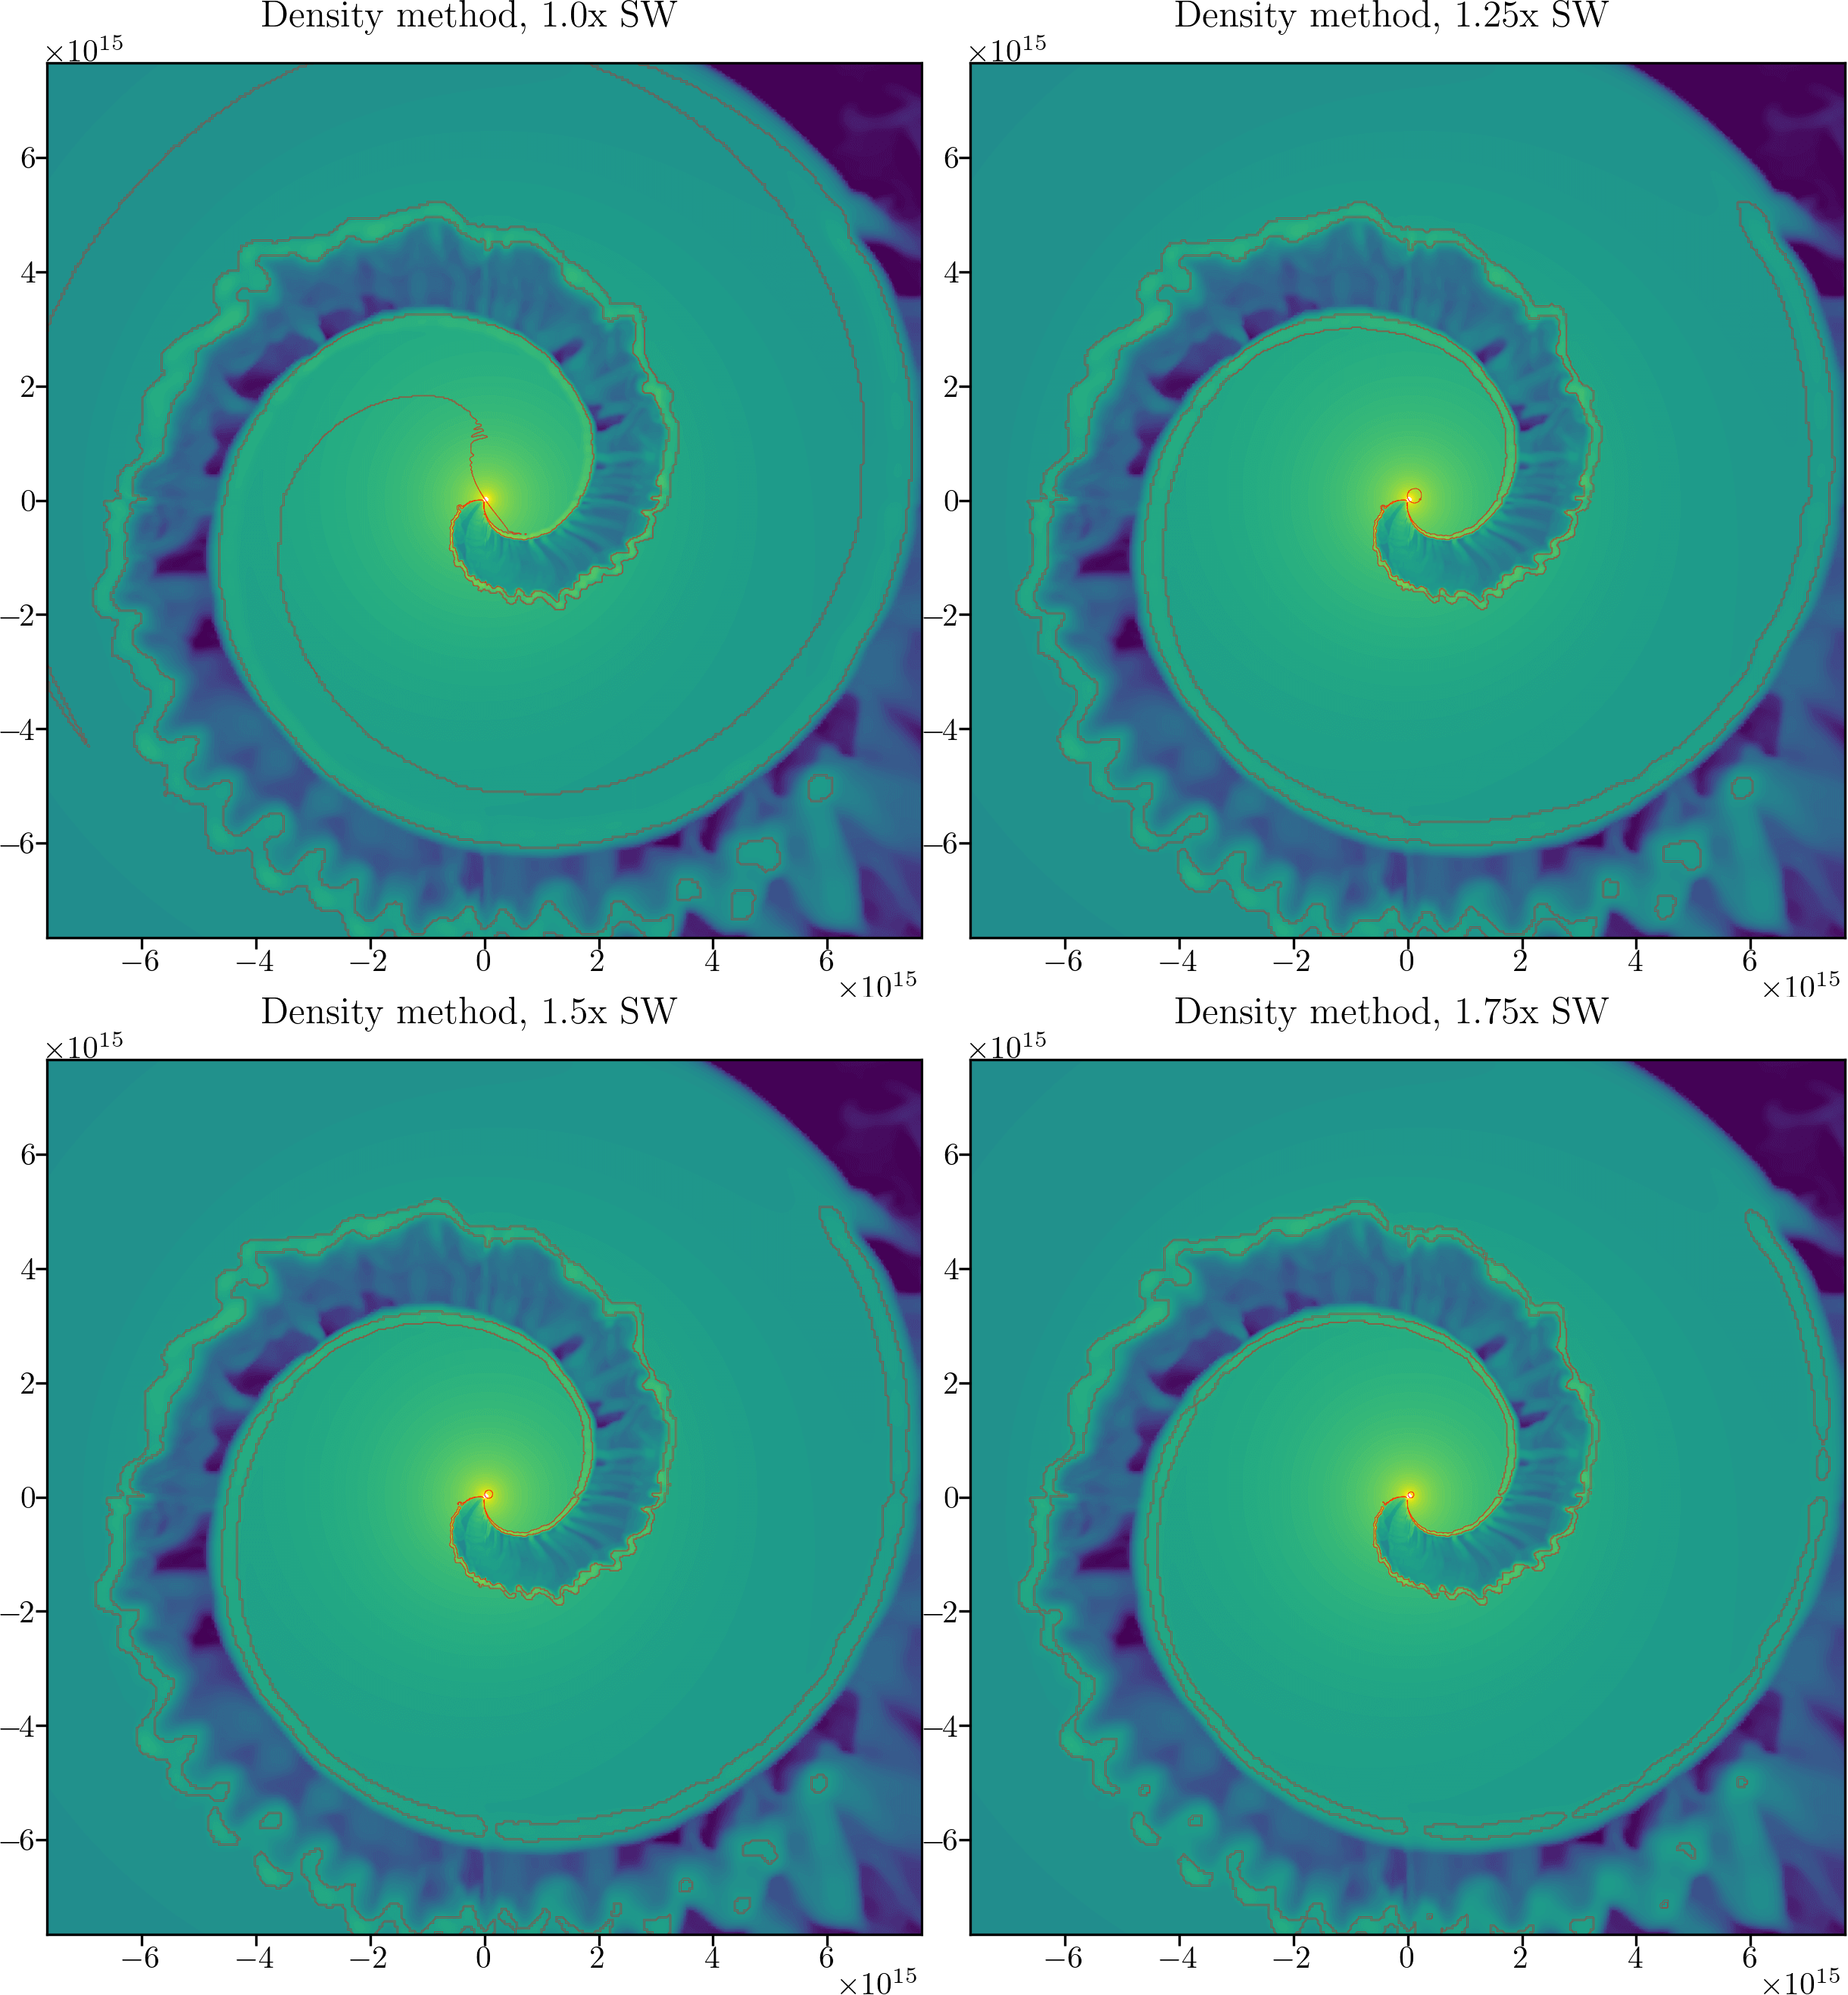
\includegraphics[width=5in]{assets/overdensity-method.png}
  \caption[Comparison of threshold values for over-density method]{Comparison of threshold values for over-density method of determining of a cell resides in the wind collision region, a threshold value of $1.25\rho_\text{SW}$ was chosen as it most accurately determined if the cell was in the post-shock region.}
  \label{fig:overdensity-threshold}
\end{figure}

\section{Results}

\subsection{Radiative processes}

\subsection{Momentum ratio variation}

\subsection{Separation variation}

% Adiabatic flow 

The most immediately apparent result to this 

%//FIXME this needs work! 32AU result is instead labelled as 64AU and zooms aren't consistent!

\begin{figure}
  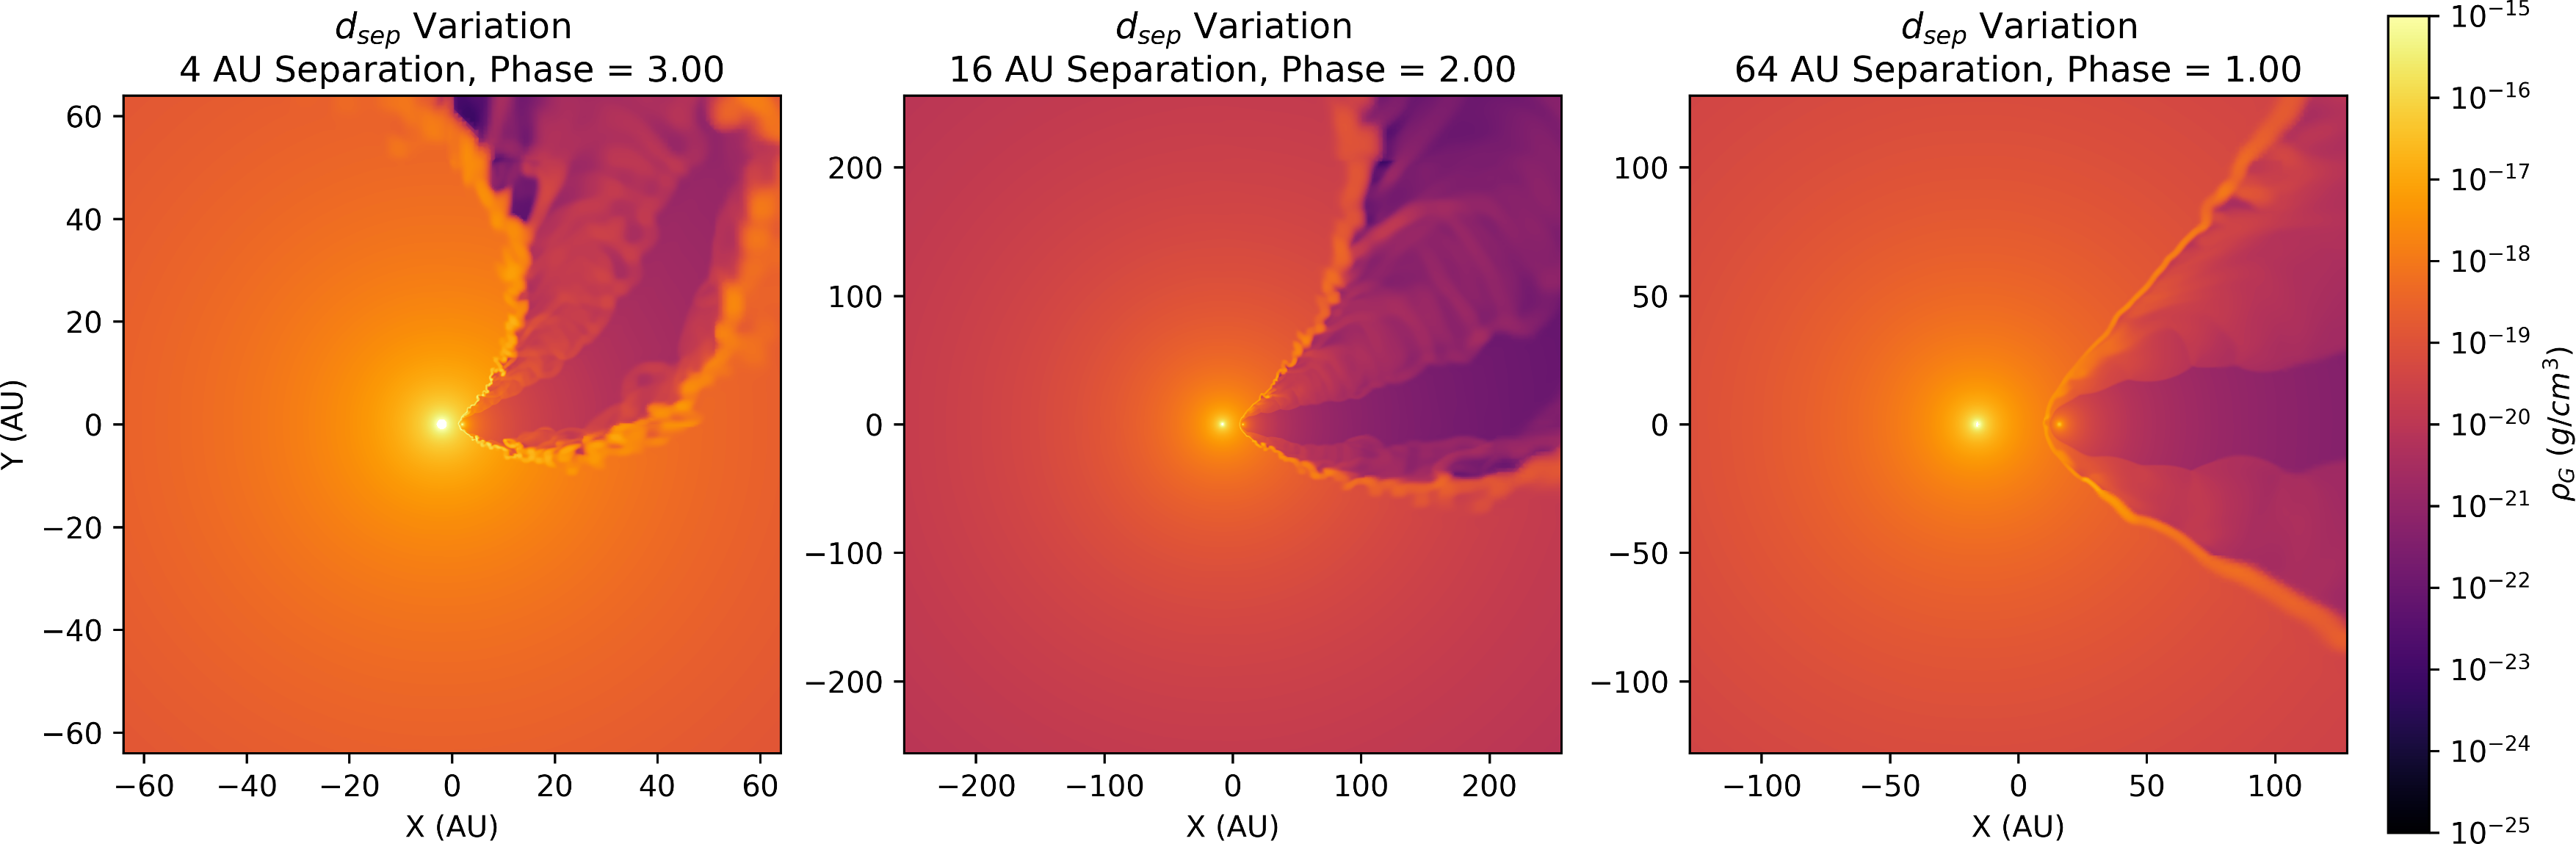
\includegraphics[width=\textwidth]{assets/adiabatic-flow/adiabatic-flow-a4.png}
\end{figure}

% Dust yields

A clear trend with orbital separation is that dust formation increases drastically as the stars are positioned closer together, at high degrees of separation dust formation ceases, and average grain size drops below the initial value of $50 \text \AA$.

The bulk of dust growth occurs in the immediate post shock region, as dust is rapidly cooled and at a high enough density for dust formation to occur.

This matches observations of episodic dust forming systems, where infrared emission due to dust is maximised at or shortly after periastron passage. This also lends further evidence that dust formation rates are not influenced solely by the momentum ratio, as this is kept constant, and instead is strongly influenced by the wind density at collision and post-shock cooling. 

% Periodicity

Closer orbits were also observed to cause subtle periodic changes, whilst this effect is less pronounced than in a highly eccentric system, the 


\subsection{Wind mixing within the WCR}

%This may need additional work

While interaction between Hydrogen and dust grains is not simulated by the dust model, \cite{leteuffModelDustFormation2002} notes that Hydrogen could be a potential catalyst for amorphous carbon grain formation.


% \appendix
% \section{Derivation of Dust Accretion and Destruction Rates}\label{app:accretiondestruction}

% \subsection{Dust destruction}\label{app:destruction}
